\lez{3}{27-02-2020}{}
Per completare il quadro dei coefficienti dobbiamo aggiungere, nel caso dell'emissione isotropa si usa il coefficiente di emissività $\epsilon _{\nu}$. Il coefficiente di emissività è l'analogo del coefficiente di emissione per unità di massa. \\
Nel caso di radiazione isotropa il legame tra questo coefficiente ed il coefficiente di emissione può essere espresso mediante la seguente:
\[
	j _{\nu} = \frac{\epsilon _{\nu} \rho }{4\pi}
.\] 
Quindi in tal caso possiamo esprimere la variazione di energia come:
\[
	dE = j _{\nu}dVdtd\Omega d\nu= \epsilon_{\nu}\rho dV dt \frac{d\Omega}{4\pi}dV
.\] 
Inoltre abbiamo la sezione d'urto $\sigma _{\nu} $ delle particelle che assorbono fotoni, possiamo dimostrare che questa è legato a $\alpha _{\nu} $. Prendiamo il volumetto di materiale attraversato:
\begin{figure}[H]
    %This is a custom LaTeX template!
    \centering
    \incfig{dimostrazione-sigma-nu}
    \caption{\scriptsize Elemento infinitesimo di materiale attraversato.}
    \label{fig:dimostrazione-sigma-nu}
\end{figure}
\noindent
Abbiamo gia definito la quantità di energia sottratta al fascio dal materiale:
\[
	dE = \alpha _{\nu} I_{\nu} dV dt d\Omega d\nu 
.\] 
Immaginiamo che il nostro mezzo sia costituito da particelle tutte uguali e tutte in grado di assorbire la radiazione, supponiamo che la sezione d'urto di assorbimento di ogni particella sia $\sigma _{\nu} $. Le particelle per unità di volume saranno: $dN = n dV = n dA ds$. Nelle ipotesi in cui il gas sia sufficientemente rarefatto:
\[
	\sqrt{\sigma _{\nu}} \ll d
.\] 
Con d distanza tra le particelle. Possiamo immaginare che le particelle del gas non si occultino l'una con l'altra, quindi la superficie assorbente complessiva sarà la somma di tutte le sezioni d'urto di ogni singola particella. Essendo le particelle tutte uguali otteniamo che $dA' = \sigma _{\nu} dN = \sigma _{\nu} dA ds$.\\
Abbiamo detto che un fotone viene assorbito su $\sigma _{\nu} $, allora nel volumetto i fotoni che vengono assorbiti sono solo quelli che incidono sulla superficie $dA'$. L'energia che viene sottratta al fascio dal materiale sarà quella che incide su questa superficie $dA'$ e visto che l'energia che attraversa tale superficie può sempre essere espressa tramite:
\[
	dE_{sott} = I_{\nu} dA' dt d\Omega d\nu 
.\] 
Possiamo eguagliare questa all'energia persa per assorbimento:
\[
	dE = \alpha _{\nu} dN dt d\Omega d\nu 
.\] 
ottenendo la legge:
\[
	\alpha_{\nu} = n \sigma_{\nu}
.\] 
Un'altra quantità utilizzata è l'opacità radiativa $k_{\nu}$, questa è legata ad $\alpha_{n}$ tramite: $\alpha_{\nu}= k_{\nu}\cdot \rho$. Questa quantità è una sezione d'urto per unità di massa, calcolarla è molto difficile.\\
Torniamo adesso alla quantità $j _{\nu} $, con questa valutiamo la quantità di radiazione che viene immessa nel fascio grazie a processi di emissione e non di scattering.\\
Quando un atomo viene eccitato può diseccitarsi in due modi:
\begin{itemize}
	\item Emissione spontanea
	\item Emissione indotta
\end{itemize}
Quindi in generale dovremmo scrivere due contributi alla $j _{\nu} $:
\[
	j _{\nu} = j _{\nu}^{\text{spont}} + j _{\nu}^{\text{ind}}
.\] 
Nel caso di emissione spontanea, nel riferimento di queite dell'atomo, l'emissione è isotropa. Inoltre in questo caso l'emissione è indipendente dalla radiazione incidente che può, di fatto, non esserci.\\
Viceversa l'emissione indotta ha bisogno della radiazione per avvenire, se sull'atomo eccitato arriva un fotone avente energia esattamente uguale all'energia di transizione di livello allora l'atomo si diseccita e libera un fotone. Il fotone emesso ha le stesse caratteristiche del fotone incidente: stessa direzione e stessa frequenza.\\
Mentre l'emissione spontanea è indipendente dal campo di radiazione l'emissione indotta non è indipendente dal camopo di radiazione.\\
Quindi di solito teniamo nell'equazione di trasporto solo il coefficiente dovuto all'emissione spontanea all'interno di $j _{\nu} $, il termine di emissione stimolata invece lo si scarica all'interno di $\alpha $ come termine negativo. In questo modo di crea un coefficiente di assorbimento corretto per l'emissione stimolata.\\
Quindi il coefficiente di assorbimento complessivo può essere positivo o negativo a seconda del processo prevalente: se prevale l'assorbimento il coefficiente darà globalmente positivo (affievolendo il fascio), se il coefficiente è negativo allora prevale l'emissione stimolata ed il fascio verrà amplificato.\\
Un esempio in cui il fascio viene amplificato per emissione stimolata sono sicuramente i laser, mentre in natura esistono oggetti chiamati Maser: sorgenti di emissione nelle microonde che si creano nelle nubi stellari, le condizioni per avere un Maser si verificano soltanto nella prima fase di vita e nell'ultima di una stella.\\
Per poter trattare l'equazione del trasporto siamo costretti a fare alcune semplificazioni. La prima e che noi considereremo sempre situazioni stazionarie, di conseguenza l'equazione diventa:
\[
	\frac{\partial I_{\nu}}{\partial s} =
	j _{\nu} 
	- \alpha_{\nu}I_{\nu} 
	- \alpha_{\nu}^{\text{scatt}}I_{\nu} 
	+ \alpha_{\nu}^{\text{scatt}} \int\phi\left( \hat{k},\hat{k}' \right) I_{\nu}\left( \hat{k}' \right) d\Omega
.\] 
Inoltre per adesso abbandioniamo lo scattering, lo riprenderemo più avanti nel corso.
\[
	\frac{\partial I_{\nu}}{\partial s} =
	j _{\nu} 
	- \alpha_{\nu}I_{\nu} 
	- \alpha_{\nu}^{\text{scatt}}I_{\nu} 
.\] 
\paragraph{Esempio: Mezzo in grado di emettere ma non di assorbire}%
In questo caso abbiamo $\alpha_{\nu}=0$, quindi l'equazione diventa:
\[
	\frac{\mbox{d} I_{\nu}}{\mbox{d} s} = j _{\nu}
.\] 
Integrando in $s$ otteniamo:
\[
	I_{\nu}\left( s \right) = I_{\nu}\left( s_0 \right) + \int_{s_0}^{s} j _{\nu}\left( s' \right) ds' > I_{\nu} ( s_0) 
.\] 
\paragraph{Esempio: Mezzo in grado di assorbire ma non di emettere}%
Al contrario del caso precedente qui abbiamo $j _{\nu}=0$, da cui: 
\[
	\frac{\mbox{d} I_{\nu}}{\mbox{d} s} = -\alpha_{\nu} I_{\nu}
.\] 
Quindi \[
	\frac{dI_{\nu}}{I_{\nu}}= -\alpha_{\nu}ds
.\] 	
\[
	I_{\nu}\left( s \right) = I_{\nu}\left( s_0 \right) \exp\left[- \int_{s_0}^{s}\alpha_{\nu}\left( s' \right) ds' \right]  
.\] 
In questo caso l'intensità della radiazione sorgente viene attenuata o incrementata a seconda del segno di $\alpha _{\nu} $.\\
Notiamo inoltre che l'esponente dell'ultima relazione è adimensionale, possiamo definirla come profondità ottica $\tau _{\nu} $.
Tale grandezza segue la relazione: 
\[
	d\tau_{\nu}= \alpha_{\nu}ds
.\] 
Vedremo che tramite questo coefficiente si semplificherà moltissimo l'equazione del trasporto.
\[
	\tau_{\nu} = \int_{s_0}^{s} \alpha_{\nu}\left( s' \right) ds'
.\] 
Dato un mezzo con una certa dimensione caratteristica $L$ la profondità ottica potrà essere molto diversa al variare della frequenza.\\
Il mezzo considerato potrà essere otticamente sottile per certe frequenze mentre potrà essere spessa per altre frequenze.\\
Viceversa se vogliamo "vedere" un mezzo con una certa profontità ottica allora l'oggetto avrà spessori ottici differenti al variare di $\nu $.\\
Tale quantità ha a che fare con il grado di trasparenza del mezzo. Posso esprimere quindi la soluzione dell'ultimo esempio in termini di $\tau_{\nu}$ :
\[
	I_{\nu}\left( \tau _{\nu}  \right) = I_{\nu}\left( s_0 \right) e^{-\tau_{\nu}}
.\] 
Se un mezzo è otticamente sottile si ha che: $\tau_{\nu}\ll 1$, quindi :
\[
	I_{\nu}\left( \tau _{\nu}  \right) \approx I_{\nu}\left( 0 \right) 
.\] 
Che significa che la radiazione arriva è la stessa della sorgente, quindi il mezzo si può considerare otticamente trasparente.\\
Viceversa se un mezzo è otticamente spesso $\tau_{\nu}\ll 1$:
\[
	I_{\nu}\approx 0
.\] 
Quindi in questo caso il mezzo è opaco, non riusciamo più a vedere la luce proveniente dalla sorgente.\\
Facciamo una piccola digressione sui livelli energetici dell'idrogeno prima di continuare la nostra trattazione.
\subsection{Serie dell'atomo di idrogeno}%
\begin{figure}[H]
	\centering
	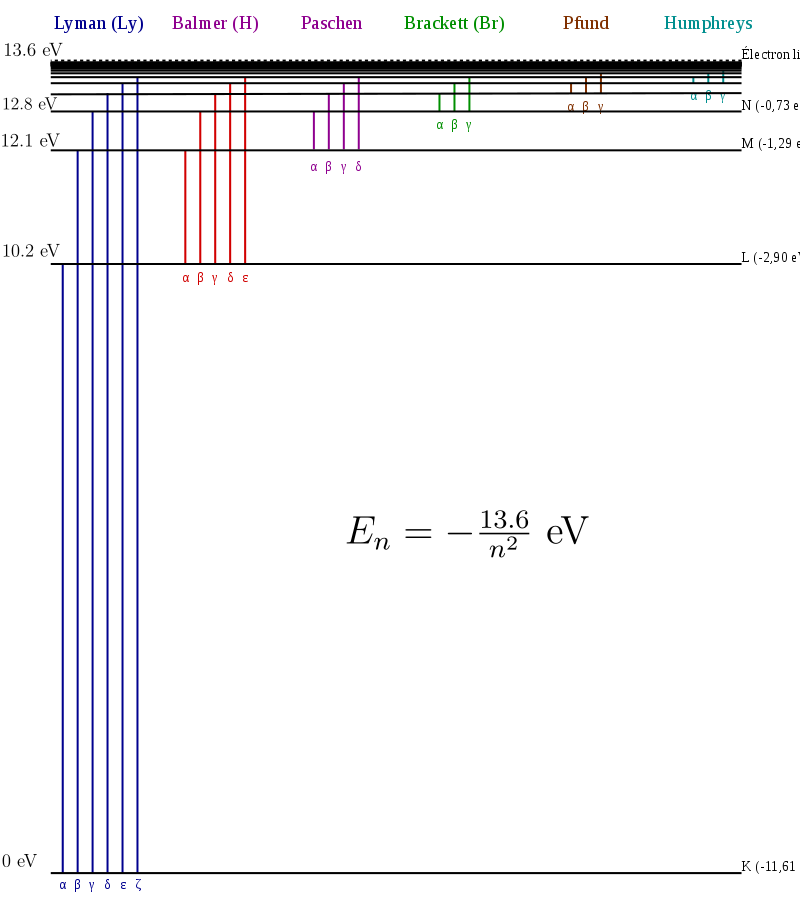
\includegraphics[width=0.5\textwidth]{figures/serie_idrogeno.png}
	\caption{\scriptsize Serie spettrale dell'idrogeno}
	\label{fig:-figures-serie_idrogeno-png}
\end{figure}
I livelli dell'atomo di idrogeno prendono la forma della Figura \ref{fig:-figures-serie_idrogeno-png}, possiamo notare diverse serie di energie che descrivono i livelli, ognuna avente il suo nome caratteristico.\\
Se mettiamo per comodità lo zero dell'energia sullo stato fondamentale abbiamo che i livelli energetici seguono la serie scritta in Figura \ref{fig:-figures-serie_idrogeno-png}.\\
Immaginiamo di voler far avvenire una transizione energetica dell'elettrone nell'idrogeno, a seconda del livello di partenza l'energia necessaria seguirà una determinata serie:
\begin{align}
	n=1 \ \to \ m \ge 2 \ &\implies \ \text{ Assorbimento da Lyman}\\
	n=2 \ \to m\ge 3 \ &\implies \ \text{ Assorbimento da Balmer} \\
			   &\ldots
.\end{align}
Il passaggio invece "dall'alto al basso" sarà l'emissione nelle varie serie.\\ 
Per la Lyman $\alpha $ ad esempio si ha che, se si emette o si assorbe un fotone dal primo stato eccitato al fondamentale (o viceversa) si ha che:
\begin{align}
	&\ce{n = 1 <-> n = 2 }  & E_{L_{\gamma \alpha }} = 10.2 \text{ eV}& &\lambda = 1216 \text{\AA}
.\end{align}
Mentre per la Lymann $\beta $:
\begin{align}
	&\ce{n = 1 <-> n = 3 }  & E_{L_{\gamma \beta  }} = 12.1 \text{ eV}& &\lambda = 1020 \text{\AA}
.\end{align}
E così via fino al salto di Lymann
\begin{align}
	&\ce{n = 1 <-> n = \infty }  & E_{L_{\infty}} = 13.6 \text{ eV}& &\lambda = 912 \text{\AA}
.\end{align}
Vediamo che questa serie è tutta nell'ultravioletto, questo è importante e dobbiamo tenerlo a mente.\\
Un'altra serie importante è la Balmer:
\begin{align}
	&\ce{n = 2 <-> n = 3 }  & E_{H_{\alpha }} = 1.9 \text{ eV}& &\lambda = 6563 \text{\AA}
.\end{align}
E così via fino al salto di Balmer:
\begin{align}
	&\ce{n = 2 <-> n = \infty }  & E_{H_{\infty }} = 3.5 \text{ eV}& &\lambda = 3646 \text{\AA}
.\end{align}
È utile notare che la serie di Balmer parte dal rosso e arriva all'ultravioletto con il salto, quindi gran parte della serie sta nel visibile, quindi quelle di Balmer sono le righe che possiamo vedere tecnicamente anche ad occhio nudo.
\subsection{Radiazione attraverso una nube interstellare}%
Ipotizziamo che il mezzo sia una nube di mezzo interstellare composta da idrogeno. La temperatura della nube è quella tipica di queste nubi: $T \approx 100$ K. Spariamo sulla nube due fasci aventi energie diverse:
\begin{align}
	&L_{\gamma,\alpha} \\
	&H_{\alpha}
.\end{align}
Ci chiediamo adesso se la nube sarà trasparente oppure opaca ai fasci inviati.\\
Se l'atomo di idrogeno si trova nello stato fondamentale allora il fotone dell'$H_{\alpha}$ non può essere assorbito, non ha l'energia per fare il salto, quindi tutti gli atomi di idrogeno sono invisibili per un fotone della $H_{\alpha}$. \\
Il fotone della $L_{\gamma,\alpha}$ invece ha l'esatta energia per effettuare il salto, quindi viene assorbito. \\
È quindi è importante capire se ci sono e quanti sono gli atomi nel primo eccitato, perchè se ci sono allora $H_{\alpha}$ viene assorbito avente l'esatta energia per permettere il salto. \\
Per capire se $H_{\alpha }$ viene assorito dalla nube è necessario capire in che stato si trovano gli atomi della nube.\\
Procediamo quindi assumendo che la nube sia all'equilibrio termodinamico e cerchiamo il rapporto tra gli atomi del primo eccitato e quello fondamentale con la distribuzione di Boltzmann:
\[
	\frac{n_2}{n_1} = \frac{g_2}{g_1}\exp\left( -\frac{\Delta E_{1,2}}{kT} \right) 
.\] 
Le $g$ sono le degenerazioni dell'atomo di idrogeno (i pesi statistici): $g_{n}= 2 n^2$ mentre $n_2$ è il numero di atomi di idrogeno che si trovano nel primo eccitato, $n_1$ è il numero di quelli che si trovano nel fondamentale. \\
Abbiamo che $ \ g_2 = 8 \ $, $ \ g_1 = 2 \ $,  $ \ \Delta E _{1,2}= 10.2 \ $eV, $ \ kT =\frac{1}{120} \ $ eV \footnote{Per ricordare questa si può ricordare che a temperatura ambiente kT = $\frac{1}{40}$ eV, quindi si ricava anche alla nostra temperatura. Sulla superficie del sole, con temperature dell'ordine di 6000 K, sarà circa mezzo eV (emissione nel visibile). Nel centro del sole invece, con circa 16 milioni di K, si ha $kT \approx$ 1 keV (emissione nell'X).}.\\
\[
	\frac{n_2}{n_1} = 4 \exp\left( - \frac{10.2}{1 / 120} \right)  = 4 \exp\left( -1224 \right) = 4\cdot 10^{-1224 /2.3} \approx 10^{-532}
.\] 
Dove abbiamo usato il fattore di conversione tra esponenziali nelle due basi.\\
Abbiamo un atomo nell'eccitato ogni $10^{532}$ atomi nel fondamentale. Bisonga capire quanti atomi ha la nube per dire se il numero di atomi che si trovano effettivamente nel primo eccitato non è trascurabile. \\
Per risolvere la questione basta però notare che $10^{532}$ sono troppi atomi persino per l'universo stesso!
\paragraph{Stima del numero di atomi nell'universo}%
La massa del sole è $2 \cdot 10^{33} $ g, la massa dell'idrogeno $M_{H} = 1.66 \cdot 10^{-24}$ g quindi il numero di atomi nel sole sarà dell'ordine di $n_{_{\odot}} = 10^{57}$, nella galassia ci sono circa $10^{11}$ stelle, quindi il numero di particelle idrogenoidi nella galassia potrebbe essere dell'ordine di $n_{\text{galassia}} \approx 10^{68}$. 
Visto che ci sono nell'universo visibile abbiamo circa $10^{11}$ galassie, quindi in tutto nell'universo visibile possiamo stimare circa $n_{\text{universo}} \approx 10^{80}$ atomi. 
Un numero incredibiblmente più piccolo di quello trovato da noi sopra.\\
Tornando all'esercizio possiamo stare molto tranquilli sul fatto che nella nube non ci saranno idrogeni nel primo eccitato, saranno tutti nel fondamentale, quindi la nube è otticamente sottile al fascio $H_{\alpha}$ anche se fosse estesa per milioni di chilometri.\\
Viceversa i fotoni della $L_{\alpha }$ verranno assorbiti, la nube sarà opaca a questi fotoni.\\
Questo ci anticipa anche che se in un mezzo come quello sopra gli atomi si eccitano (tipicamente per collisioni) e si diseccitano successivamente nella $H_{\alpha }$ allora i fotoni emessi usciranno dal mezzo indisturbati portando con se dell'energia. 
Questo è una tecnica di raffreddamento per il mezzo stesso che può perdere energia per collisioni e successiva emissione.\\
Inoltre se andiamo sul sito dell'hubble space telescope e cerchiamo le regioni di formazione stellare $H_2$ vediamo delle regioni di un colore rossastro, questo è proprio $H_{\alpha }$ che, con i suoi $6563$ \AA $ \ $  esce dalla nube per arrivare alla lente di Hubble.
\begin{figure}[H]
	\centering
	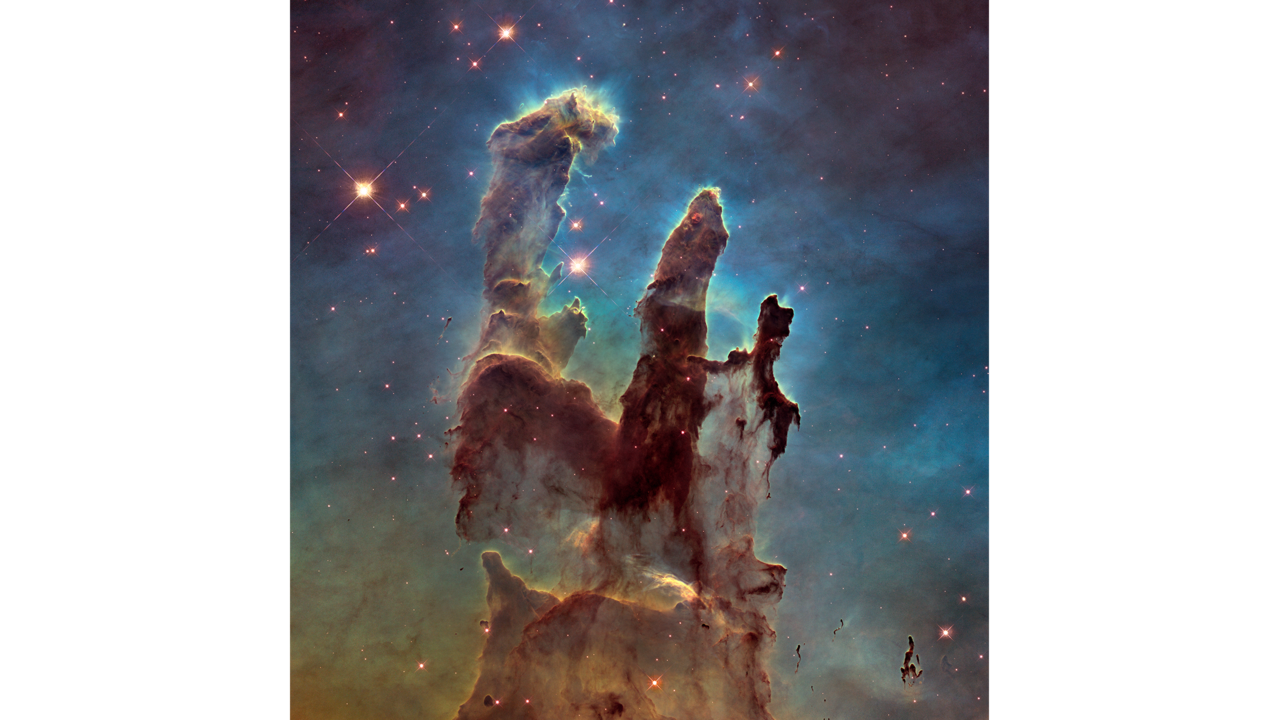
\includegraphics[width=0.8\textwidth]{figures/veil-nebula.png}
	\caption{\scriptsize Immagine di una nebulosa nel visibile (modificata per accentuare la nitidezza).}
	\label{fig:figures-veil-nebula-png}
\end{figure}
\noindent
\subsection{Soluzione analitica all'equazione del trasporto stazionaria.}%
Abbiamo visto che l'espressione dell'equazione del trasporto in condizioni stazionarie si riduce a:
\[
	\frac{\mbox{d} I_{\nu}}{\mbox{d} s} = j _{\nu} - \alpha_{\nu}I_{\nu} 
.\] 
Vogliamo fare un cambio di variabile, anzichè studiarla rispetto alla variabile $s$ la vogliamo rispetto alla profondità ottica $\tau _{\nu} $.
\[
	\frac{\mbox{d} I_{\nu}}{\mbox{d} s} = \frac{\mbox{d} I_{\nu}}{\mbox{d} \tau_{\nu}} \frac{\mbox{d} \tau_{\nu}}{\mbox{d} s} = \frac{\mbox{d} I_{\nu}}{\mbox{d} \tau_{\nu}} \alpha_{\nu} = j _{\nu} - \alpha_{\nu}I_{\nu}
.\]
L'equazione modificata diventa:
\[
	\frac{\mbox{d} I_{\nu}}{\mbox{d} \tau_{\nu}}  = \frac{j _{\nu}}{\alpha_{\nu}}- I_{\nu}
.\] 
Possiamo allora definire il primo termine dopo l'uguale come:
\begin{defn}[Funzione sorgente]{def:Funzione sorgente}
	Il rapporto tra il coefficiente di emissione ed il coefficiente di assorbimento è detto funzione sorgente $s_{\nu} $:
	\[
		s_{\nu} = \frac{j _{\nu} }{\alpha _{\nu} }
	.\] 
\end{defn}
L'equazione del trasporto con questo termine è ovviamente:
\[
	\frac{\mbox{d} I_{\nu}}{\mbox{d} \tau_{\nu}} = s_{\nu}- I_{\nu}
.\] 
Possiamo notare inoltre che 
\[
s_{\nu}<I_{\nu} \implies \frac{\mbox{d} I_{\nu}}{\mbox{d} \tau_{\nu}} <0
.\]
In questo modo l'intensità del fascio viene attenuata nell'attraversare la nube. Viceversa:
\[
s_{\nu}>I_{\nu} \implies \frac{\mbox{d} I_{\nu}}{\mbox{d} \tau_{\nu}} >0
.\]
Quindi il fascio viene amplificato nel passagio.\\
Proviamo a risolvere formalmente l'equazione:
\[
	\frac{\mbox{d} I_{\nu}}{\mbox{d} \tau_{\nu}}e^{\tau_{\nu}} = s_{\nu}e^{\tau_{\nu}}- I_{\nu}e^{\tau_{\nu}}
.\] 
Quindi possiamo raggruppare:
\[
	\frac{\mbox{d} }{\mbox{d} \tau _{\nu} } \left( I_{\nu}e^{\tau_{\nu}} \right) = s_{\nu}e^{\tau_{\nu}}
.\] 
e integriamo tra 0 e $\tau _{\nu} $:
\[
	\int_{0}^{\tau_{\nu}}\frac{\mbox{d} }{\mbox{d} \tau'_{\nu}} \left( I_{\tau'_{\nu} } e^{\tau' _{\nu} } \right) d\tau '_{\nu}  = 
	\int_{0}^{\tau _{\nu} } s( \tau '_{\nu} ) e^{\tau '_{\nu} }d\tau _{\nu} 
.\] 
integrando il primo termine ottiene: 
\[
	I_{\nu}\left( \tau_{\nu} \right) e^{\tau_{\nu}} - I_{\nu}\left( 0 \right) = 
	\int_{0}^{\tau_{\nu}} s_{\nu}\left( \tau_{\nu}' \right) e^{\tau_{\nu}'}d \tau_{\nu}'
.\] 
Se dividiamo tutto per $e^{\tau _{\nu} }$ abbiamo la legge per $I_{\nu} ( \tau _{\nu} ) $.
\begin{fact}[Soluzione formale all'equazione del trasporto]{fact:Soluzione formale all'equazione del trasporto}
	\[
	I_{\nu}\left( \tau_{\nu} \right) = I_{\nu}\left( 0 \right)e^{-\tau_{\nu}} - \int_{0}^{\tau_{\nu}} \delta_{\nu}\left( \tau_{\nu}' \right) e^{-(\tau_{\nu}-\tau_{\nu}')}d \tau_{\nu}'
.\] 
\end{fact}
Il primo termine è la luce della sorgente estinta esponenzialmente dal mezzo a causa dell'assorbimento. Il secondo termine contiene il significato fisico di due distinti effetti: l'effetto dell'emissione di fotoni del fascio nei vari punti del mezzo ($s_{\nu} $) e l'effetto dell'assorbimento incluso nel termine esponenziale.\\
Innfatti il termine $\tau _{\nu} -\tau '_{\nu} $ sta ad indicare l'assorbimento dei fotoni che sono stati emessi dal mezzo. \\
Anche se abbiamo la soluzione generale resta il fatto che $s_{\nu} $ è incognita, anche se conoscessimo l'espressione analitica di $s_{\nu} $ non saremo comunque in grado di calcolare l'integrale poichè non conosciamo le condizioni fisiche (pressione, temperatura \ldots) del mezzo \footnote{dalle quali ricordiamo dipendere $\tau _{\nu} $}.
\paragraph{Esempio: mezzo omogeneo.}%
Se il mezzo è omogeneo per tutta la sua estensione si mantengono costanti le sue proprietà fisiche. Di conseguenza avremo che $\alpha _{\nu} $ e $j _{\nu} $ saranno uguali ovunque e la funzione sorgente sarà anch'essa una costante:
\[
	I_{\nu}\left( \tau_{\nu} \right) = I_{\nu}\left( 0 \right) e^{-\tau_{\nu}} + s_{\nu} e^{-\tau_{\nu}}\int_0^{\tau_{\nu}} e^{\tau_{\nu}'}d \tau_{\nu}' =
	I_{\nu}\left( 0 \right) e^{-\tau_{\nu}} + s_{\nu}\left( 1-e^{-\tau_{\nu}} \right) \label{eq:soluzione-mezzo-omogeneo}
.\] 
Possiamo iniziare ad intuire il significato fisico della funzione sorgente:
se il nostro fascio attraversa un mezzo otticamente profondo ($\tau_{\nu}\rightarrow \infty$) allora abbiamo che $I_{\nu}\left( \tau_{\nu} \right) \rightarrow s_{\nu}$. Allora la funzione sorgente è la grandezza fisica a cui tende l'intensità della radiazione se questa attraversa una regione otticamente spessa. Quindi ciò che succede al fascio in questo caso è una totale sostituzione dei fotoni provenienti dalla sorgente con i fotoni emessi all'interno del mezzo come in Figura \ref{fig:soluzione-all-equazione-del-trasporto-per-mezzo-otticamente-spesso}
\begin{figure}[H]
    %This is a custom LaTeX template!
    \centering
    \incfig{soluzione-all-equazione-del-trasporto-per-mezzo-otticamente-spesso}
    \caption{\scriptsize Sostituzione dei fotoni in un mezzo otticamente spesso.}
    \label{fig:soluzione-all-equazione-del-trasporto-per-mezzo-otticamente-spesso}
\end{figure}
\noindent
Man mano che la radiazione si propaga i fotoni del fascio perderanno le caratteristiche della radiazione sorgente ed acquisteranno invece la firma del mezzo.\\
Notiamo che questo non è soltanto un processo astrofisico, questo avviene anche quando guardiamo delle montagne lontane che ci appaiono celestine come il cielo:
\begin{figure}[H]
	\centering
	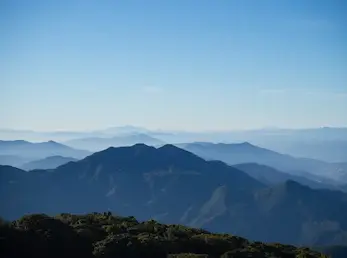
\includegraphics[width=0.4\textwidth]{figures/farmountain.png}
	\caption{\scriptsize Montagne lontane che acquistano il colore del cielo fino a dissolversi con esso.}
	\label{fig:figures-farmountain-jpg}
\end{figure}

\paragraph{Esempio: Mezzo omogeneo senza retroilluminazione}
In questo caso particolare abbiamo che $I_{\nu} ( 0) = 0$, l'unica radiazione che vediamo emergere è quella prodotta dal mezzo stesso.
\[
	I_{\nu} ( \tau _{\nu} ) = s_{\nu}\left( 1-e^{-\tau _{\nu} } \right)  
.\] 
Consideriamo adesso i casi in cui il mezzo è otticamene sottile o spesso alla radiazione che emerge da lui stesso.
\subparagraph{Mezzo otticamente sottile}
Siamo in questa situazione se $\tau _{\nu} \ll 1$, sviluppiamo l'esponenziale:
\[
	I_{\nu} ( \tau _{\nu} ) = s_{\nu} \tau _{\nu} 
.\] 
Visto che il mezzo è omogeneo si ha:
\[
	\tau _{\nu} = \int_{s_0}^{s} \alpha _{\nu} ( s') ds'= \alpha _{\nu} ( s-s_0)  = \alpha _{\nu} \cdot L
.\] 
Quindi abbiamo che:
\[
	I_{\nu} ( \tau _{\nu} ) = s_{\nu} \alpha _{\nu}\cdot  L = j _{\nu} \cdot L
.\] 
Dalla quale emerge l'importante contributo alla radiazione di $j _{\nu} $ in questa situazione.\\
Se il mezzo è costituito da atomi non completamente ionizzati allora sappiamo che la radiazione ha dei picchi in intensità molto marcati in corrispondenza della frequenza di transizione dei livelli, quindi sia il coefficiente di assorbimento $\alpha _{\nu} $ che il coefficiente di emissione $j _{\nu} $ avranno dei picchi molto marcati in corrispondenza di queste transizioni. Quindi qua ci aspettiamo proprio questo tipo di radiazione proveniente dal "mezzo", molto marcata in corrispondenza della transizione dei livelli delle specie atomiche. \\
Questa radiazione emergente sarà perciò caratterizzato da delle righe di emissione: uno spettro buio quasi ovunque con delle righe luminose.\\
Un esempio di questo tipo è un gas rarefatto riscaldato: una lampada al neon. Un esempio nello spazio sono le nebulose. \footnote{Nelle stelle invece vedo delle righe di assorbimento miste al continuo}
\subparagraph{Mezzo otticamente spesso}
Quando scaldiamo un oggetto a temperature elevate inizia ad essere percepibile la sua emissione di radiazione termica, questo passerà in modo continuo dal rosso scuro, poi al giallo, ecc\ldots \\
Prendiamo un mezzo omogeneo non retroilluminato ed otticamente spesso $\tau _{\nu} \gg 1$, in questo limite abbiamo che:
\[
	I_{\nu} ( \tau _{\nu} )  = s_{\nu} 
.\] 
Quindi la radiazione che emerge è uguale alla funzione sorgente, questo è il caso del oggetto riscaldato. Infatti la funzione sorgente è parente della radiazione di corpo nero che è una funzione della temperatura. Quindi in questo caso abbiamo uno spettro continuo.\\
Nel cosmo oggetti che approssimeranno questa radiazione sono le stelle, non sara esattamente una radiazione di corpo nero perchè abbiamo delle righe di assorbimento. Studieremo prossimamente da dove vengono queste misteriose righe di assorbimento.
